\documentclass[14pt]{extreport}
\usepackage{gost}



\begin{document}
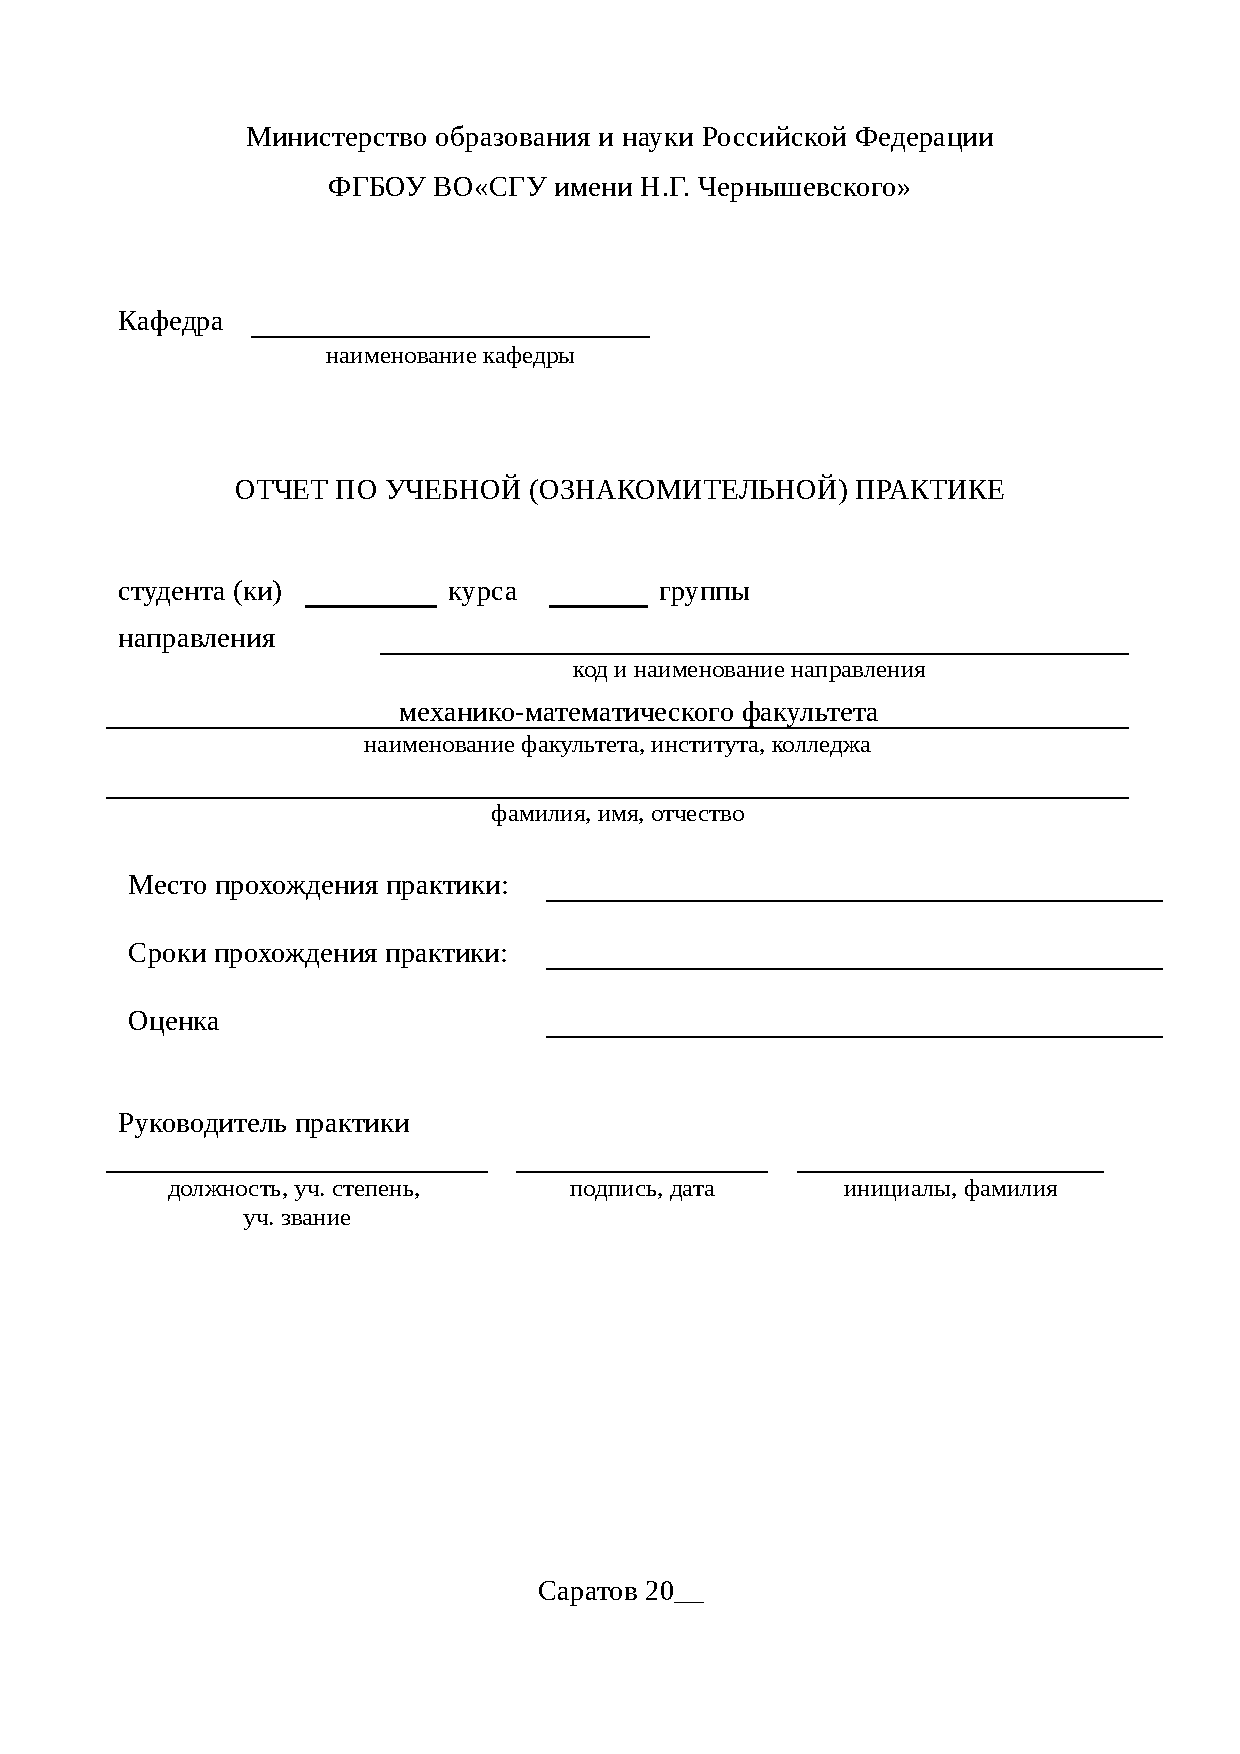
\includepdf[pages={1}]{titulOzPrac.pdf}


\tableofcontents

\intro

Ознакомительная практика является неотъемлемой частью учебного процесса. Студентам необходима подготовка к осознанному и углубленному изучению общепрофессиональных и специальных дисциплин и получение навыков самостоятельной практической работы по сбору фактического материала, составлению базы данных для различных исследований, анализа собранной информации.

\chapter{Множества. Действительные числа}

\section{Основные понятия}

Под множеством понимают совокупность (собрание, класс, семейство...) некоторых объектов, объединенных по какому-либо признаку.
Множество обозначается заглавными буквами, например $M$, $X$. Прописными латинскими буквами обозначаются элементы множеств, например $a$, $x$.

\section{Числовые множества. Множества действительных чисел}

\section{Числовые промежуткию Окрестность точки}



\chapter{Функция}

\section{Числовые функции. График функции}

\section{Обратная функция}

\section{Сложная функция}



\chapter{Последовательности}

\section{Числовая последовательность}

\section{Предел числовой последовательности}

\section{Предельный переход в неравенствах}

\section{Предел монотонной ограниченной последовательности. Число $e$. Натуральные логарифмы}



\chapter{Предел функции}

\section{Предел функции в точке}

\section{Односторонние пределы}

\section{Предел функции при $x\to\infty$}

\section{Бесконечно большая функция}



\chapter{Бесконечно малые функции}

\section{Определения и основные теоремы}

\section{Связь между функцией, ее пределом и бесконечно малой функцией}

\section{Основные теоремы о пределах}

\section{Признаки существования пределов}

\section{Первый замечательный предел}

\section{Второй замечательный предел}



\chapter{Эквивалентные бесконечно малые функции}

\section{Сравнение бесконечно малых функций}

\section{Эквивалентные беконечно малые и основные теоремы о них}

\section{Применение эквивиалентных бесконечно малых функций}



\chapter{Непрерывность функций}

\section{Непрерывность функции в точке}

\section{Непрерывность функции в интервале и на отрезке}

\section{Точки разрыва функции и их классификация}

\section{Основные теоремы о непрерывных функциях. Непрерывность элементарных функций}

\section{Свойства функций непрерывных на отрезке}



\chapter{Производная функции}


























\end{document}